\section{RF and M/W Transmission Lines}
{\color{sub}\footnotesize 6 hrs \gap$\cdot$\gap asked in \mk{all 24 papers}
\gap$\cdot$\gap \mk{297 marks}, 12.4 per paper \gap$\cdot$\gap 4 syllabus sub-topics
$\rightarrow$ the Smith chart chapter: almost every mark here is a graphical construction.}

\vspace{3pt}\noindent
\colorbox{gdL}{\makebox[\dimexpr\textwidth-2\fboxsep][l]{%
  \textcolor{gd}{\bfseries\footnotesize READ THIS FIRST}}}
\par\nobreak\vspace{3pt}

This is the second-heaviest chapter in the subject and the most predictable one.
Of its 297 marks, roughly 230 are stub-matching constructions, and
\textbf{double-stub tuning alone appears in 17 of the 24 papers} --- the single most
reliably asked item in RF and Microwave Engineering. Learn the construction, not the answers.
\begin{enumerate}[label=\arabic*., leftmargin=1.4em, itemsep=1pt]
  \item \textbf{Double-stub matching} (17 papers, usually 8--12 marks) $\rightarrow$ master
    one procedure: spacing circle, constant-$g$ arc, rotate, cancel. It works for every
    variant the examiner prints (stub spacing $\lambda/8$ or $3\lambda/8$, short or open,
    first stub at the load or offset).
  \item \textbf{The S-matrix rider} (10 papers) $\rightarrow$ ``prepare the S-matrix of the
    matched network'' is tacked onto most stub questions and is worth 2--6 marks for two
    lines of work. See \S2.8; do not leave it.
  \item \textbf{Single-stub matching} (6 papers) and \textbf{the immittance chart}
    (5 papers) $\rightarrow$ both are short, self-contained and frequently the easy half of
    a long question.
\end{enumerate}
Numerical work is in the companion, \textit{Ch2 --- RF and MW Transmission Lines ---
Numerical Problems \& Solutions}, where all 24 PYQ constructions are solved step by step.

\hr

%=======================================================================
\T{2.1 Types of Transmission Lines}

\Q{Differentiate the behaviour of a transmission line at conventional low frequency and at microwave bands. Compare microwave transmission lines with conventional low-frequency lines}{\m{4}\m{5}\m{10}}
{\color{sub}\footnotesize \tF{3} \yr{\textbf{69 Bh}, 71 Ma, \textbf{79 Ch}} \gap$\cdot$\gap builds on \S1.2; here the focus is the \emph{line} rather than the circuit}

\sbs{%
\lead{A transmission line is a guiding structure}
\begin{itemize}
  \item At low frequency, power is thought of as travelling \textbf{in the wire}; the pair
    of conductors merely completes a circuit.
  \item At microwave frequency, power travels \textbf{in the $\vec{E}$ and $\vec{H}$ fields}
    between and around the conductors. Any structure that guides that field from place to
    place is a transmission line.
  \item The governing criterion is again $d/\lambda$ (\S1.2): once the line length is a
    noticeable fraction of $\lambda$, voltage and current are functions of position.
\end{itemize}
\lead{Classification}
\begin{itemize}
  \item \textbf{Two-conductor (TEM) lines} --- support a pure TEM mode, no low-frequency
    cut-off:
  \begin{itemize}
    \item Two-wire open line, twisted pair (UTP / STP), coaxial cable, stripline.
  \end{itemize}
  \item \textbf{Quasi-TEM lines} --- inhomogeneous dielectric, so no exact TEM:
  \begin{itemize}
    \item Microstrip, coplanar waveguide (CPW), slot line, fin line.
  \end{itemize}
  \item \textbf{Single-conductor (waveguide) lines} --- TE/TM modes only, and a
    \textbf{cut-off frequency} below which nothing propagates:
  \begin{itemize}
    \item Rectangular and circular waveguide, dielectric waveguide, optical fibre.
  \end{itemize}
  \item \textbf{Balanced vs unbalanced}: two-wire and twisted pair are balanced (equal and
    opposite currents, common-mode noise cancels); coaxial is unbalanced (signal referred
    to the grounded outer). A \textbf{balun} converts between them.
\end{itemize}
\lead{Choosing a line --- the four practical trade-offs}
\begin{itemize}
  \item \textbf{Loss}: waveguide $<$ coax $<$ microstrip at a given frequency.
  \item \textbf{Power handling}: waveguide (kW--MW) $\gg$ coax $\gg$ microstrip (W).
  \item \textbf{Bandwidth}: TEM lines are broadband; waveguide is limited by cut-off and
    the next higher mode.
  \item \textbf{Cost and integration}: microstrip is photolithographic and near-free;
    waveguide is machined and expensive.
\end{itemize}}{%
\lead{Low-frequency line vs microwave line}
\begin{tabularx}{\linewidth}{@{}L{1.75cm}X X@{}}
\toprule
\hrow \thead{Aspect} & \thead{Conventional (LF)} & \thead{RF / Microwave} \\
\midrule
\textbf{Model} & Ideal short; length irrelevant. & Distributed $R', L', G', C'$ per metre. \\
\textbf{Analysis} & KVL / KCL, lumped. & Telegrapher's equations, Maxwell. \\
\textbf{$V$, $I$} & Uniform along the line. & $v(z,t)$, $i(z,t)$; standing waves. \\
\textbf{Loss} & Ohmic ($I^2R$) only. & Conductor ($\propto\!\sqrt{f}$, skin effect), dielectric ($\tan\delta$), \emph{and} radiation. \\
\textbf{Reflection} & None considered. & At every discontinuity; measured by $\Gamma$, VSWR. \\
\textbf{Typical lines} & Wire, twisted pair, PCB trace. & Coax, waveguide, microstrip, stripline. \\
\textbf{Termination} & Matching not needed. & Must terminate in $Z_0$ or match with a tuner. \\
\textbf{Joints} & Any solder joint. & Precision connectors (SMA, N, APC-7); a bad joint is a reflector. \\
\bottomrule
\end{tabularx}
\lead{The planar family, in cross-section}
\figT{c2_planar_lines.png}
{\color{sub}\scriptsize (a) stripline, (b) microstrip, (c) slot line, (d) coplanar strips,
with $E$ (solid) and $H$ (dashed). Only (a) has one homogeneous dielectric round the conductor,
so only (a) is pure TEM. Das \& Das Fig 3.27.}}

\penalty0\vspace{2pt}

{\color{sub}\footnotesize$\rightarrow$ For \textbf{microstrip vs stripline} (asked \yr{71 Ma}),
see \S1.6 --- geometry, quasi-TEM vs pure TEM, dispersion, shielding and fabrication are
compared there and are not repeated.}

%=======================================================================
\T{2.2 Transmission Line Theory}

\Q{Derive the transmission line (telegrapher's) equations and obtain the characteristic impedance, reflection coefficient, VSWR and input impedance}{\m{4}\m{6}\m{8}}
{\color{sub}\footnotesize \tF{3} \yr{\textbf{69 Bh}, \textbf{79 Ch}, 71 Ma} \gap$\cdot$\gap the toolkit every numerical in this chapter uses}

\sbs{%
\lead{Distributed model and the telegrapher's equations}
\mbox{}\hfill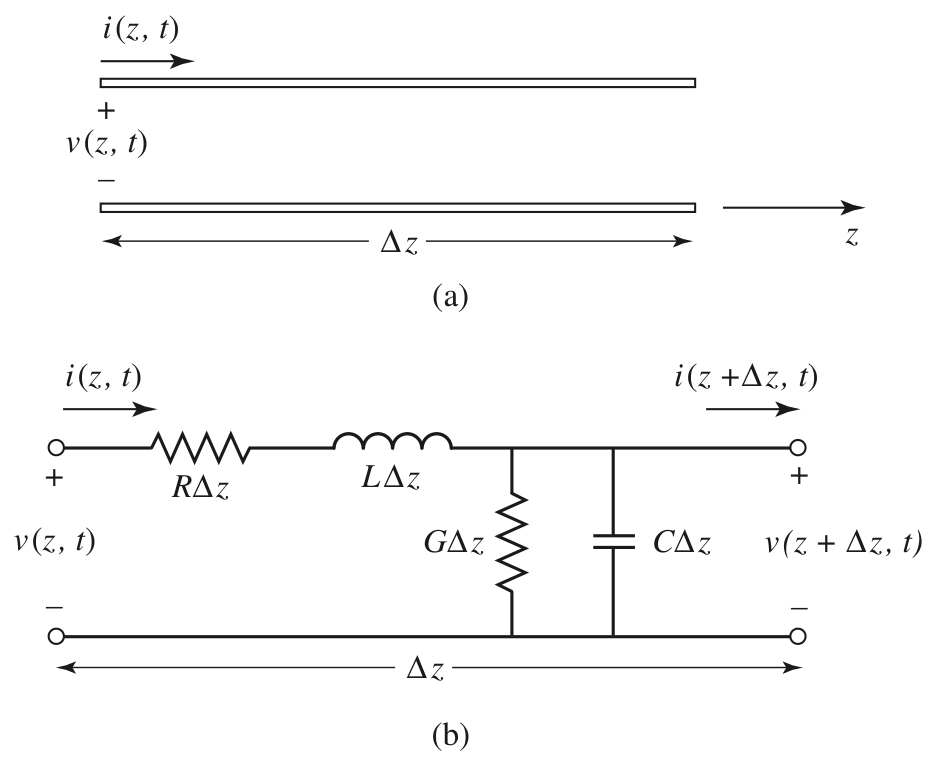
\includegraphics[width=0.62\linewidth]{figs/c2_lumped_model.png}\hfill\mbox{}\par
{\color{sub}\scriptsize (a) $v$, $i$ on a length $\Delta z$; (b) its equivalent cell. Draw (b)
before writing KVL and KCL. Pozar Fig 2.1.}
\begin{itemize}
  \item A length $\Delta z$ of line is modelled by series $R'\Delta z$, $L'\Delta z$ and
    shunt $G'\Delta z$, $C'\Delta z$, all \textbf{per unit length}.
  \item Applying KVL and KCL to that cell and letting $\Delta z \rightarrow 0$:
    \[ \frac{\partial v}{\partial z} = -R'i - L'\frac{\partial i}{\partial t},
       \qquad
       \frac{\partial i}{\partial z} = -G'v - C'\frac{\partial v}{\partial t} \]
  \item In phasor form these decouple into the \textbf{wave equations}
    \[ \frac{d^2V}{dz^2} = \gamma^2 V, \qquad \frac{d^2I}{dz^2} = \gamma^2 I \]
  \item \textbf{Propagation constant} and \textbf{characteristic impedance}:
    \[ \gamma = \alpha + j\beta = \sqrt{(R'+j\omega L')(G'+j\omega C')} \]
    \[ Z_0 = \sqrt{\frac{R'+j\omega L'}{G'+j\omega C'}} \]
  \item Solution: $V(z) = V_0^{+}e^{-\gamma z} + V_0^{-}e^{+\gamma z}$ --- a forward and a
    reflected travelling wave.
\end{itemize}
\lead{Lossless line ($R'=G'=0$) --- used for every PYQ in this chapter}
\begin{itemize}
  \item $\alpha = 0$, \quad $\beta = \omega\sqrt{L'C'}$, \quad
        $Z_0 = \sqrt{L'/C'}$ (\textbf{purely real}).
  \item $\lambda = 2\pi/\beta = v_p/f$, \quad $v_p = 1/\sqrt{L'C'} = c/\sqrt{\epsilon_r}$.
\end{itemize}
\lead{Distortionless line}
\begin{itemize}
  \item Condition: $R'C' = L'G'$. Then $\alpha = \sqrt{R'G'}$ is frequency-independent and
    $\beta = \omega\sqrt{L'C'}$ is linear in $\omega$, so all frequencies travel at the same
    $v_p$ and the pulse shape survives.
\end{itemize}}{%
\lead{Terminated line: the four quantities every problem needs}
\begin{itemize}
  \item \textbf{Load reflection coefficient}
    \[ \Gamma_L = \frac{Z_L - Z_0}{Z_L + Z_0} = \frac{z_L - 1}{z_L + 1},
       \qquad z_L = \frac{Z_L}{Z_0} \]
  \item \textbf{At a distance $d$ toward the generator}, only the phase changes on a
    lossless line:
    \[ \Gamma(d) = \Gamma_L\,e^{-j2\beta d}, \qquad |\Gamma(d)| = |\Gamma_L| \]
    This is why the Smith chart works: moving along the line is a \emph{rotation at
    constant radius}.
  \item \textbf{VSWR}
    \[ S = \frac{V_{\max}}{V_{\min}} = \frac{1+|\Gamma_L|}{1-|\Gamma_L|},
       \qquad 1 \le S \le \infty \]
  \item \textbf{Input impedance}
    \[ Z_{in}(d) = Z_0\,\frac{Z_L + jZ_0\tan\beta d}{Z_0 + jZ_L\tan\beta d} \]
  \item \textbf{Return loss} $= -20\log_{10}|\Gamma|$ dB;
    \textbf{mismatch loss} $= -10\log_{10}(1-|\Gamma|^2)$ dB.
\end{itemize}
\lead{Special line lengths --- memorise these}
\begin{tabularx}{\linewidth}{@{}L{2.15cm}X@{}}
\toprule
\hrow \thead{Case} & \thead{Input impedance} \\
\midrule
\textbf{Matched} $Z_L=Z_0$ & $Z_{in}=Z_0$ for any length; $\Gamma=0$, $S=1$. \\
\textbf{Short} $Z_L=0$ & $Z_{in} = jZ_0\tan\beta d$ --- purely reactive, inductive for $d<\lambda/4$. \\
\textbf{Open} $Z_L=\infty$ & $Z_{in} = -jZ_0\cot\beta d$ --- purely reactive, capacitive for $d<\lambda/4$. \\
\textbf{$d=\lambda/2$} & $Z_{in} = Z_L$ --- the line repeats every half wavelength. \\
\textbf{$d=\lambda/4$} & $Z_{in} = Z_0^2/Z_L$ --- the \textbf{quarter-wave transformer}; it \emph{inverts}, so a short looks open. \\
\textbf{$d=\lambda/8$} & $Z_{in} = Z_0\,\dfrac{Z_L+jZ_0}{Z_0+jZ_L}$ \quad ($\tan\beta d = 1$). \\
\bottomrule
\end{tabularx}
\vspace{2pt}
{\footnotesize\color{sub} A shorted or open stub is therefore a \emph{pure reactance whose
value you choose by cutting it to length} --- that single fact is the whole basis of stub
matching.}}

\penalty0\vspace{2pt}

%=======================================================================
\T{2.3 The Smith Chart}

\Q{Explain the construction of the Smith chart. What does each family of curves represent, and how is it read?}{\m{4}\m{5}\m{10}}
{\color{sub}\footnotesize \tF{5} \yr{\textbf{72 Ash}, \textbf{75 Bh}, 72 Ma, \texttt{81 Ba}, \textbf{80 Ch}} \gap$\cdot$\gap counted together with the immittance chart in \S2.4}

\sbsr{0.52}{%
\lead{What the chart is}
\begin{itemize}
  \item A plot of \textbf{normalised impedance $z = r + jx$ mapped onto the complex
    $\Gamma$ plane} by the bilinear transform
    \[ \Gamma = \frac{z-1}{z+1}, \qquad z = \frac{1+\Gamma}{1-\Gamma} \]
  \item Because $|\Gamma| \le 1$ for a passive load, the entire right half of the $z$ plane
    folds into the \textbf{unit circle} --- an infinite plane on one sheet of paper.
\end{itemize}
\lead{The two families of curves}
\begin{itemize}
  \item \textbf{Constant resistance $r$}: circles centred on
    $\left(\dfrac{r}{1+r},\,0\right)$ with radius $\dfrac{1}{1+r}$.
    All pass through the open-circuit point $\Gamma = +1$.
  \item \textbf{Constant reactance $x$}: arcs centred on
    $\left(1,\,\dfrac{1}{x}\right)$ with radius $\left|\dfrac{1}{x}\right|$.
    Upper half $= +x$ (\textbf{inductive}), lower half $= -x$ (\textbf{capacitive}).
  \item The two families are \textbf{orthogonal} everywhere they cross.
\end{itemize}
\lead{Landmarks}
\begin{itemize}
  \item \textbf{Centre} $z=1$: matched, $\Gamma=0$, $S=1$.
  \item \textbf{Left} $z=0$: short circuit, $\Gamma=-1$.
  \item \textbf{Right} $z=\infty$: open circuit, $\Gamma=+1$.
  \item \textbf{Rim} $|\Gamma|=1$: pure reactance, total reflection, $S=\infty$.
  \item Horizontal axis: $x=0$, i.e. purely resistive. To the right of centre lies
    $V_{\max}$ (and $r = S$); to the left lies $V_{\min}$ (and $r = 1/S$).
\end{itemize}
\lead{Reading it --- the five rules}
\begin{enumerate}[label=\arabic*., leftmargin=1.4em]
  \item Normalise: $z_L = Z_L/Z_0$. Plot it.
  \item $|\Gamma_L|$ = distance from centre $\div$ chart radius; its angle is read on the
    \textbf{angle of reflection coefficient} scale.
  \item Draw the \textbf{constant-$|\Gamma|$ (SWR) circle} through the point. Read $S$ where
    it cuts the right-hand real axis.
  \item \textbf{Move toward the generator = clockwise}; toward the load $=$ anticlockwise.
    \textbf{One full lap is $\lambda/2$}, so a quarter turn is $\lambda/8$.
  \item Read distances on the \textbf{WTG} (wavelengths toward generator) rim scale, which
    runs $0 \rightarrow 0.5$ clockwise starting at the short-circuit point.
\end{enumerate}}{%
\figT{c2_smith_blank.png}
{\footnotesize\color{sub} The impedance chart. Constant-$r$ circles (all through the open
point) and constant-$x$ arcs; the rim carries the WTG scale, on which one complete lap is
half a wavelength of line.}}

\penalty0\vspace{2pt}

\lead{Why the chart is worth using at all}
\begin{itemize}
  \item It turns the awkward $Z_{in}$ formula into a \textbf{rotation}, and $z \rightarrow y$
    into a \textbf{half-turn} --- both done with a compass instead of complex arithmetic.
  \item $\Gamma$, $S$, $Z_{in}$, $Y_{in}$, return loss and the positions of $V_{\max}$ and
    $V_{\min}$ are all read off one diagram.
  \item It shows \emph{graphically} which matching solutions exist, and lets you pick the
    one with the shortest stub or the widest bandwidth --- something a formula does not
    show you.
\end{itemize}

\penalty0\vspace{2pt}

%=======================================================================
\T{2.4 The Immittance (Admittance) Chart}

\Q{Sketch an immittance chart. List the duality parameters and compare the two scales}{\m{2}\m{4}\m{5}\m{10}}
{\color{sub}\footnotesize \tF{5} \yr{\textbf{72 Ash}, \textbf{75 Bh}, 72 Ma, \texttt{81 Ba}, \textbf{80 Ch}} \gap$\cdot$\gap short, self-contained, and asked five times}

\sbsr{0.52}{%
\lead{The admittance chart}
\begin{itemize}
  \item Since $y = 1/z$, and
    \[ \Gamma_y = \frac{y-1}{y+1} = -\frac{z-1}{z+1} = -\Gamma_z \]
    the admittance chart is \textbf{the impedance chart rotated through
    $180^\circ$} (a $\lambda/4$ line length).
  \item So on a plain Smith chart you convert $z \rightarrow y$ by drawing a diameter
    through the point and reading the diametrically opposite intersection.
\end{itemize}
\lead{The immittance chart}
\begin{itemize}
  \item \textbf{Both grids printed on one chart}, usually in two colours: the impedance
    grid and the admittance grid superimposed.
  \item A single location then carries \textbf{two readings at once} --- $z$ on one grid,
    $y$ on the other. The $\lambda/4$ half-turn is built into the printing.
  \item \textbf{Why it matters}: stub matching is done in \emph{admittance} (shunt stubs
    add susceptance) but loads are quoted as \emph{impedance}. Without an immittance chart
    every problem costs an extra half-turn, and each half-turn is a chance to misread.
\end{itemize}
\lead{Duality parameters}
\begin{tabularx}{\linewidth}{@{}L{2.5cm}X@{}}
\toprule
\hrow \thead{Impedance grid} & \thead{Admittance grid} \\
\midrule
$z = r + jx$ & $y = g + jb$ \\
Resistance $r$ & Conductance $g$ \\
Reactance $x$ & Susceptance $b$ \\
$+x$ inductive (upper) & $+b$ \textbf{capacitive} (upper) \\
$-x$ capacitive (lower) & $-b$ \textbf{inductive} (lower) \\
Short $z=0$ at $\Gamma=-1$ & Open $y=0$ at $\Gamma=-1$ \\
Open $z=\infty$ at $\Gamma=+1$ & Short $y=\infty$ at $\Gamma=+1$ \\
Series elements add & Shunt elements add \\
$r=1$ circle & $g=1$ circle \\
\bottomrule
\end{tabularx}
\vspace{2pt}
{\footnotesize\color{sub}\textbf{Trap.} The sign convention flips: a point in the
\emph{upper} half is inductive read as an impedance but \emph{capacitive} read as an
admittance. Both are the same physical point.}}{%
\figT{c2_immittance.png}
{\footnotesize\color{sub} Immittance chart. The amber grid is the blue grid turned through
$180^\circ$; one location reads $z = 0.5+j0.7$ on the impedance grid and
$y = 0.68-j0.95$ on the admittance grid. The faint point is where $y$ would have to be read
on a plain chart --- a $\lambda/4$ turn away.}}

\penalty0\vspace{2pt}

%=======================================================================
\T{2.5 Impedance Matching: Why, and Which Technique}

\Q{Why is impedance matching necessary? Compare the different impedance matching techniques}{\m{4}\m{5}\m{6}}
{\color{sub}\footnotesize \tF{3} \yr{\textbf{78 Ch}, 74 Ma, \textbf{77 Ch}} \gap$\cdot$\gap the theory half of several double-stub questions}

\sbs{%
\lead{Why match}
\begin{itemize}
  \item \textbf{Maximum power transfer}: a matched load absorbs all incident power;
    the fraction reflected is $|\Gamma|^2$.
  \item \textbf{Protect the source}: reflected power returning to a high-power amplifier or
    a magnetron causes heating, and can destroy it.
  \item \textbf{Remove standing waves}: high VSWR means voltage peaks that cause dielectric
    breakdown and arcing, and current peaks that cause $I^2R$ loss.
  \item \textbf{Preserve receiver sensitivity}: mismatch at an LNA input degrades the noise
    figure directly.
  \item \textbf{Avoid distortion}: multiple reflections on a long line arrive delayed,
    producing ghosting and intersymbol interference.
\end{itemize}
\lead{The matching network must be lossless}
\begin{itemize}
  \item A resistive pad would ``match'' but dissipate the very power being matched.
  \item So matching uses only \textbf{reactive} elements: line lengths, stubs, lumped
    $L$ and $C$.
\end{itemize}
\figT{c2_lossless_match.png}
{\color{sub}\scriptsize The general problem: a lossless network between line $Z_0$ and load
$Z_L$, chosen so the line sees $Z_0$. Every technique in the table is one way to build the box.
Pozar Fig 5.1.}}{%
\lead{Comparison of techniques}
\begin{tabularx}{\linewidth}{@{}L{2.05cm}X X@{}}
\toprule
\hrow \thead{Technique} & \thead{How it works} & \thead{Trade-offs} \\
\midrule
\textbf{Quarter-wave transformer} & $\lambda/4$ of line with $Z_{01}=\sqrt{Z_0 Z_L}$. & Simplest, but \textbf{needs a real $Z_L$} --- a complex load must first be walked to a $V_{\max}$ or $V_{\min}$. Narrowband. \\
\textbf{L-section (lumped)} & Two reactances, series $+$ shunt. & Compact; fine below $\sim$1 GHz. Above that, component parasitics (\S1.3) dominate. \\
\textbf{Single stub} & One shunt (or series) stub at a computed distance $d$. & Matches \textbf{any} load; only line, so no lumped parts. \textbf{But $d$ must move if the load changes} --- awkward to build as an adjustable tuner. \\
\textbf{Double stub} & Two stubs at \textbf{fixed} spacing; only the lengths are tuned. & Positions are pre-set, so it makes a practical \textbf{adjustable} tuner. \textbf{But a range of loads cannot be matched} (the forbidden region). \\
\textbf{Triple stub} & Three fixed stubs. & Removes the forbidden region entirely; used in laboratory slide-screw tuners. \\
\bottomrule
\end{tabularx}
\vspace{2pt}
\lead{Advantages of double stub over single stub}
\begin{itemize}
  \item Stub \textbf{positions are fixed}; matching is done by adjusting lengths only, so
    it can be built as a mechanical tuner with two sliding shorts.
  \item No need to break into the line at a computed distance --- the connection points are
    decided at manufacture.
  \item Retunes for a new load without physically relocating anything.
  \item \textbf{Cost}: a set of load admittances (the forbidden region) is unmatchable, and
    two stubs mean a slightly narrower bandwidth.
\end{itemize}}

\penalty0\vspace{2pt}

%=======================================================================
\T{2.6 Single-Stub Tuning}

\Q{Explain the design of a single-stub shunt tuner, stating all steps with reasoning. When is a short-circuited stub preferred over an open one?}{\m{8}\m{10}\m{2+8}}
{\color{sub}\footnotesize \tF{6} \yr{\textbf{72 Ash}, \textbf{74 Bh}, 72 Ma, \textbf{76 Bh}, \textbf{79 Ch}, \textbf{\texttt{81 Bh}}} \gap$\cdot$\gap worked instances in the numerical companion}

\sbs{%
\lead{Principle}
\begin{itemize}
  \item Two degrees of freedom are needed to cancel a complex mismatch, and a single stub
    supplies exactly two: \textbf{the distance $d$ from the load to the stub}, and
    \textbf{the stub length $\ell$}.
  \item Work in \textbf{admittance}, because a shunt stub \emph{adds} its susceptance:
    \[ y_{in} = y(d) + y_{stub} = 1 + jb + (-jb) = 1 \]
  \item \textbf{Step 1 --- choose $d$} so the line admittance has unit conductance:
    $y(d) = 1 + jb$. Geometrically, walk round the SWR circle until it cuts the
    \textbf{$g=1$ circle}. It always cuts it \textbf{twice}, so there are always
    \emph{two} solutions.
  \item \textbf{Step 2 --- choose $\ell$} so the stub presents $-jb$, cancelling the
    residual susceptance and leaving $y_{in}=1$, i.e. $Z_{in}=Z_0$.
\end{itemize}
\lead{Design procedure on the chart}
\begin{enumerate}[label=\arabic*., leftmargin=1.4em]
  \item Normalise $z_L = Z_L/Z_0$ and plot it.
  \item Half-turn to $y_L$ (or read it on the admittance grid). Note its WTG reading.
  \item Draw the SWR circle through $y_L$.
  \item Move \textbf{clockwise} to each intersection with the $g=1$ circle; call them
    $y_1 = 1 - jb$ and $y_2 = 1 + jb$. The WTG difference from $y_L$ gives $d_1$ and $d_2$.
  \item The stub must supply $+jb$ and $-jb$ respectively.
  \item For the stub length, start at the \textbf{termination point of the stub} --- the
    open-circuit point ($y=0$) for an open stub, the short-circuit point ($y=\infty$) for a
    shorted stub --- and run \textbf{clockwise round the rim} to the required susceptance.
    That arc, read on the WTG scale, is $\ell$.
\end{enumerate}}{%
\lead{Analytic check (use it to verify the chart)}
\begin{itemize}
  \item With $t = \tan\beta d$ and $Z_L = R_L + jX_L$, the distance satisfies
    \[ t = \frac{X_L \pm \sqrt{R_L\big[(Z_0-R_L)^2 + X_L^2\big]/Z_0}}{R_L - Z_0} \]
    reducing to $t = -X_L/2Z_0$ when $R_L = Z_0$.
  \item Then $d/\lambda = \dfrac{1}{2\pi}\tan^{-1}t$ (add $0.5$ if negative).
  \item \textbf{Stub length from the required susceptance $b_s$}:
    \[ \frac{\ell_{open}}{\lambda} = \frac{1}{2\pi}\tan^{-1}(b_s), \qquad
       \frac{\ell_{short}}{\lambda} = \frac{-1}{2\pi}\tan^{-1}\!\left(\frac{1}{b_s}\right) \]
    always reduced modulo $0.5\lambda$.
\end{itemize}
\lead{Short-circuited or open-circuited stub?}
\begin{tabularx}{\linewidth}{@{}L{1.55cm}X@{}}
\toprule
\hrow \thead{Stub} & \thead{When it is preferred} \\
\midrule
\textbf{Short} & \textbf{Coax and waveguide.} A shorting plate is exact and radiates nothing; an open coax end radiates and has fringing capacitance, so its electrical length is not its physical length. Also easier to make adjustable (sliding short). \\
\textbf{Open} & \textbf{Microstrip and other planar lines.} Ending the strip is free; a true short needs a via drilled and plated through the substrate, which adds inductance and cost. \\
\bottomrule
\end{tabularx}
\vspace{2pt}
{\footnotesize\color{sub} The two lengths differ by exactly $\lambda/4$:
$\ell_{short} = \ell_{open} \pm \lambda/4$.}
\vspace{2pt}
\lead{Which of the two solutions to build}
\begin{itemize}
  \item Prefer the \textbf{smaller $d$}: less line between load and stub means a shorter
    high-VSWR section, hence lower loss and \textbf{wider bandwidth}.
  \item Prefer the \textbf{shorter stub} for the same reason, and for compactness.
  \item A series stub is used when the line cannot be shunted (some waveguide and
    coaxial geometries); the construction is identical but done on the \emph{impedance}
    grid against the $r=1$ circle.
\end{itemize}}

\penalty0\vspace{3pt}
\sbsr{0.56}{%
\lead{The circuit, which is what to draw}
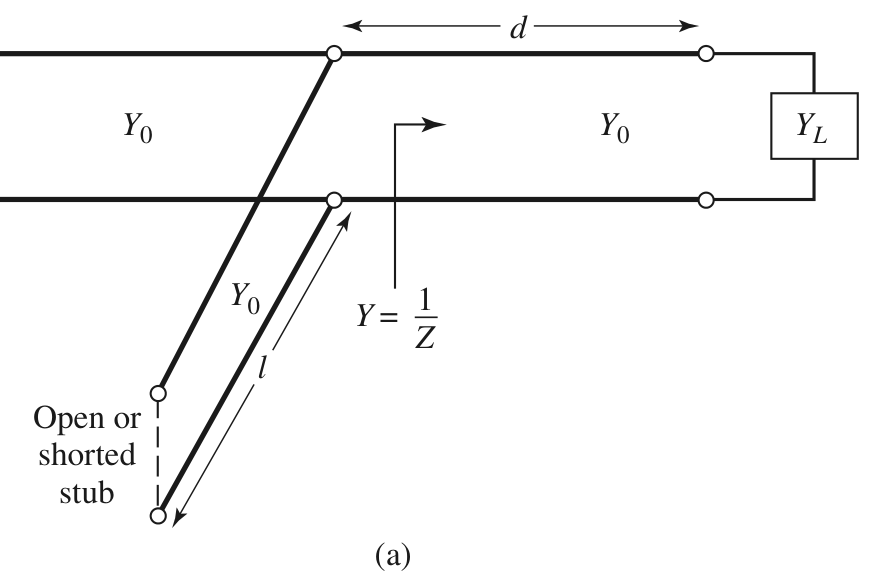
\includegraphics[width=0.49\linewidth]{figs/c2_single_stub_a.png}\hfill
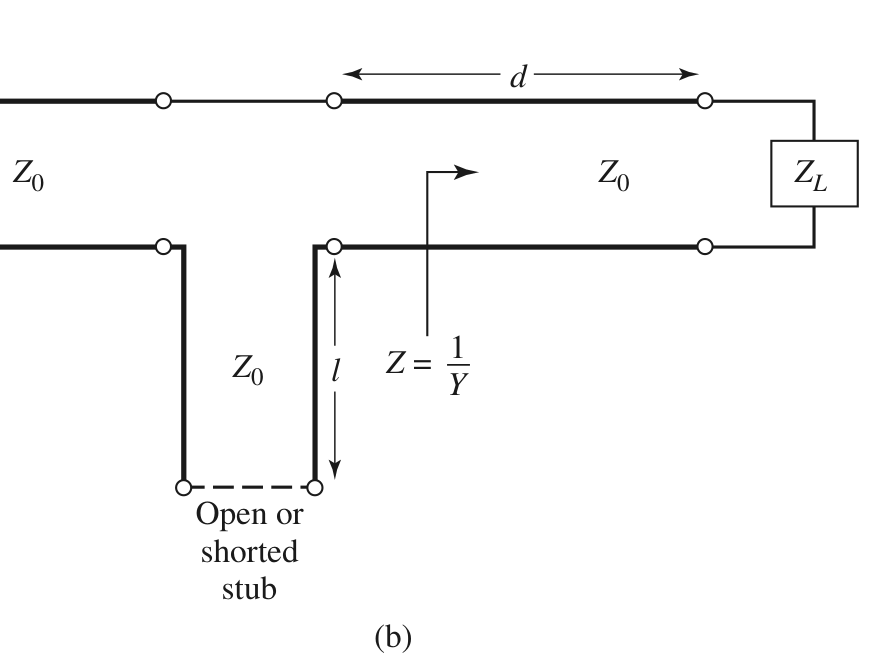
\includegraphics[width=0.49\linewidth]{figs/c2_single_stub_b.png}}{%
\vspace{2pt}
\begin{itemize}
  \item \textbf{(a) Shunt stub}: at distance $d$ from the load the line admittance is
    $Y = 1/Z = Y_0 + jB$; the stub of length $\ell$, open or shorted, adds $-jB$.
  \item \textbf{(b) Series stub}: same two unknowns $d$ and $\ell$, but the stub is in series,
    so work in impedance: $Z = Z_0 + jX$ at $d$, stub supplies $-jX$.
  \item Mark $d$ from the \textbf{load} and $\ell$ from the stub's \textbf{open or shorted
    end} on the sketch: those are the two answers the question asks for.
  \item Pozar Fig 5.4.
\end{itemize}}

\penalty0\vspace{2pt}

%=======================================================================
\T{2.7 Double-Stub Tuning}

\Q{Explain the steps for impedance matching of a load using a double-stub network. State the advantages over single-stub matching and the limitation of the technique}{\m{8}\m{10}\m{12}\m{2+8}}
{\color{sub}\footnotesize \tS{17} \yr{\textbf{69 Bh}, \textbf{70 Bh}, 70 Ma, \textbf{71 Bh}, \textbf{73 Bh}, 73 Ma, 74 Ma, \textbf{75 Bh}, \textbf{77 Ch}, \textbf{78 Ch}, \textbf{80 Ch}, \texttt{80 Ba}, \textbf{\texttt{80 Bh}}, \texttt{81 Ba}, \textbf{\texttt{79 Bh}}, \texttt{82 Ba}, \textbf{\texttt{82 Bh}}} \gap$\cdot$\gap \mk{the single most asked item in the subject}}

\sbs{%
\lead{Principle}
\begin{itemize}
  \item The two stubs sit at \textbf{fixed} positions a distance $d$ apart --- almost
    always \textbf{$\lambda/8$ or $3\lambda/8$} in the papers. Only the two lengths
    $\ell_1$ and $\ell_2$ are adjusted, and those are the two degrees of freedom.
  \item \textbf{Stub 1} cannot change the conductance it sees --- a shunt susceptance moves
    the point \emph{along its own constant-$g$ circle}. Its job is to land the point where
    the intervening $d$ of line will carry it onto the $g=1$ circle.
  \item \textbf{Stub 2} then simply cancels whatever susceptance is left, exactly as in
    single-stub matching.
\end{itemize}
\lead{The spacing circle --- the key construction}
\begin{itemize}
  \item Define the \textbf{spacing circle} as the $g=1$ circle rotated $d$
    \textbf{toward the load} (anticlockwise).
  \item Any point on it is carried \emph{onto} $g=1$ by $d$ wavelengths of line.
  \item So stub 1 must move the point from $y_1$ to the intersection of its own
    constant-$g$ circle with the spacing circle. There are generally \textbf{two}
    intersections, hence two solutions.
\end{itemize}
\lead{Design procedure}
\begin{enumerate}[label=\arabic*., leftmargin=1.4em]
  \item Normalise $z_L$, plot, half-turn to $y_L$.
  \item If the first stub is offset from the load by $d_1$, rotate $y_L$ clockwise by $d_1$
    to get $y_1$, the admittance \emph{just before} stub 1.
  \item Draw the spacing circle ($g=1$ rotated $d$ toward the load).
  \item Follow the \textbf{constant-$g$ circle through $y_1$} to its intersections with the
    spacing circle: $y_a$ and $y_a'$.
  \item $b_1 = \operatorname{Im}(y_a) - \operatorname{Im}(y_1)$ --- the susceptance stub 1
    must add. Read $\ell_1$ off the rim from the stub's termination point.
  \item Rotate $y_a$ clockwise by $d$ along its SWR circle; it lands on $g=1$ at
    $y_2 = 1 + jb_2'$.
  \item $b_2 = -b_2'$; read $\ell_2$ off the rim the same way. The network is matched.
\end{enumerate}}{%
\lead{Analytic check}
\begin{itemize}
  \item With $y_1 = g_1 + jb_L$ and $t = \tan\beta d$, requiring
    $\operatorname{Re}(y_2)=1$ after the spacing gives
    \[ \operatorname{Re}(y_2) = \frac{g_1(1+t^2)}{(1-tB)^2 + t^2g_1^2} = 1 \]
    \[ \Rightarrow \quad B = \frac{1 \pm \sqrt{g_1(1+t^2) - g_1^2t^2}}{t},
       \qquad b_1 = B - b_L \]
    where $B$ is the total susceptance after stub 1. \textbf{Note the leading $1$ in the
    numerator, not $g_1$} --- a common slip.
  \item Then $y_a = g_1 + jB$, and
    $y_2 = \dfrac{y_a + jt}{1 + jt\,y_a}$, with $b_2 = -\operatorname{Im}(y_2)$.
\end{itemize}
\lead{The forbidden region --- always state this}
\begin{itemize}
  \item The square root is real only if
    \[ g_1 \;\le\; \frac{1}{\sin^2\beta d} \]
  \item For $d = \lambda/8$ ($\beta d = 45^\circ$): $g_1 \le 2$.
    \\ \mbox{}\hfill For $d = 3\lambda/8$: $g_1 \le 2$ likewise.
    \\ \mbox{}\hfill For $d = \lambda/4$: $g_1 \le 1$.
  \item Loads whose conductance at the first stub exceeds this \textbf{cannot be matched}
    at all with that spacing. Graphically, their constant-$g$ circle lies wholly inside the
    spacing circle and never cuts it.
  \item \textbf{The fix}: add a length of line before the first stub (which moves $g_1$), or
    use a third stub.
  \item This is why $\lambda/4$ spacing is avoided in practice and $\lambda/8$ or
    $3\lambda/8$ is used --- and why the examiner keeps specifying $3\lambda/8$.
\end{itemize}
\vspace{2pt}
{\footnotesize\color{sub}\textbf{Trap.} Stub spacings near $\lambda/2$ make the two stubs
nearly coincident and the tuner hopelessly narrowband, so practical spacings stay between
$\lambda/8$ and $3\lambda/8$.}}

\penalty0\vspace{3pt}
\sbsr{0.38}{%
\lead{The circuit, which is what to draw}
\figT{c2_double_stub.png}}{%
\vspace{2pt}
\begin{itemize}
  \item \textbf{(a)} load an arbitrary distance from the first stub: stub 1 ($jB_1$, length
    $\ell_1$) nearer the load, stub 2 ($jB_2$, $\ell_2$) a fixed $d$ further toward the
    generator.
  \item \textbf{(b)} the same tuner with that offset line absorbed into the load, now called
    $Y_L'$. This is step 2 of the procedure: rotate $y_L$ by $d_1$ first, then design as if
    stub 1 sat at the load.
  \item Only $\ell_1$ and $\ell_2$ are adjusted; $d$ is fixed at manufacture, which is the
    whole advantage over one stub.
  \item Pozar Fig 5.7.
\end{itemize}}

\penalty0\vspace{2pt}

%=======================================================================
\T{2.8 S-Matrix of a Matched Network}

\Q{Prepare the scattering matrix of the network before and after matching}{\m{2}\m{2+2}\m{4}\m{6}}
{\color{sub}\footnotesize \tS{10} \yr{\textbf{76 Bh}, \textbf{77 Ch}, \textbf{78 Ch}, \texttt{80 Ba}, \textbf{\texttt{80 Bh}}, \texttt{81 Ba}, \textbf{\texttt{81 Bh}}, \textbf{\texttt{79 Bh}}, \texttt{82 Ba}, \textbf{\texttt{82 Bh}}} \gap$\cdot$\gap \mk{free marks: two lines of work, tacked onto ten stub questions}}

\sbs{%
\lead{Before matching --- a one-port}
\begin{itemize}
  \item An unmatched load seen from the line is a \textbf{one-port}, so its scattering
    matrix is the single entry
    \[ [S] = \big[\,\Gamma_L\,\big] = \left[\frac{Z_L-Z_0}{Z_L+Z_0}\right] \]
  \item Quote it in polar form, $|\Gamma_L|\angle\theta^\circ$, and give the VSWR
    alongside --- the examiner usually wants both.
\end{itemize}
\lead{After matching --- an ideal two-port}
\begin{itemize}
  \item A perfectly matched, lossless, reciprocal two-port has
    \textbf{no reflection at either port}, so $S_{11} = S_{22} = 0$, and all power passes
    through, so $|S_{12}| = |S_{21}| = 1$:
    \[ [S] = \begin{bmatrix} 0 & 1 \\ 1 & 0 \end{bmatrix} \]
  \item Keeping the electrical length $\theta = \beta\ell$ of the through path:
    \[ [S] = \begin{bmatrix} 0 & e^{-j\theta} \\ e^{-j\theta} & 0 \end{bmatrix} \]
    Either answer earns the marks; state which convention you are using.
\end{itemize}}{%
\lead{Justifying each property (this is where the marks are)}
\begin{itemize}
  \item \textbf{$S_{11}=S_{22}=0$}: that is the definition of a match --- the tuner was
    designed to make $Z_{in} = Z_0$ looking in at either port.
  \item \textbf{Reciprocity}, $S_{12} = S_{21}$: the network contains only passive,
    isotropic media (line and stubs), no ferrite and no active device, so $[S]$ is
    symmetric, $[S] = [S]^T$.
  \item \textbf{Lossless}, so $[S]$ is \textbf{unitary}:
    $[S]^{*T}[S] = [I]$, giving $\sum_k |S_{ki}|^2 = 1$ for every column. With
    $S_{11}=0$ this forces $|S_{21}| = 1$.
  \item \textbf{Reactive elements only} means no power is dissipated, only redirected --- so
    all incident power appears at the far port.
\end{itemize}
\lead{Worked shape of the answer}
\begin{itemize}
  \item ``Before: $\Gamma_L = (Z_L-Z_0)/(Z_L+Z_0) = 0.45\angle60^\circ$, so
    $[S]=[\,0.45\angle60^\circ\,]$ and $S = 2.64$.''
  \item ``After: the tuner makes $Z_{in}=Z_0$, so $S_{11}=S_{22}=0$; the network is
    reciprocal and lossless, so $S_{12}=S_{21}$ with $|S_{21}|=1$, giving
    $[S]=\left[\begin{smallmatrix}0&1\\1&0\end{smallmatrix}\right]$.''
\end{itemize}
\vspace{2pt}
{\footnotesize\color{sub} S-parameter theory in full --- properties, derivation, shifting
reference planes --- is Chapter 3. This band covers only the rider attached to stub
questions.}}

\penalty0\vspace{2pt}

%=======================================================================
\T{2.9 Microstrip Realisation of a Stub Tuner}

\Q{Sketch the physical diagram of the matched network using microstrips}{\m{2}\m{2+2}\m{4}}
{\color{sub}\footnotesize \tF{4} \yr{\textbf{72 Ash}, 72 Ma, \textbf{77 Ch}, \texttt{82 Ba}} \gap$\cdot$\gap turns $\lambda$ answers into millimetres}

\sbs{%
\lead{From electrical length to millimetres}
\begin{itemize}
  \item Microstrip is \textbf{quasi-TEM}, so the wave sees an effective permittivity
    between air and substrate:
    \[ \epsilon_{e} = \frac{\epsilon_r+1}{2} + \frac{\epsilon_r-1}{2}
       \frac{1}{\sqrt{1+12h/W}} \]
  \item Guide wavelength, and hence every physical length:
    \[ \lambda_g = \frac{\lambda_0}{\sqrt{\epsilon_e}} = \frac{c}{f\sqrt{\epsilon_e}},
       \qquad \ell_{\text{mm}} = \frac{\ell}{\lambda}\times\lambda_g \]
  \item \textbf{Strip width} for a wanted $Z_0$ (Hammerstad synthesis), with
    $B = \dfrac{377\pi}{2Z_0\sqrt{\epsilon_r}}$ and $W/h > 2$:
    \[ \frac{W}{h} = \frac{2}{\pi}\Big[B-1-\ln(2B-1)
       + \frac{\epsilon_r-1}{2\epsilon_r}\Big(\ln(B-1)+0.39-\frac{0.61}{\epsilon_r}\Big)\Big] \]
\end{itemize}
\lead{Layout rules the examiner looks for}
\begin{itemize}
  \item Stubs are drawn as \textbf{T-junctions off the main line}, at the computed spacing.
  \item \textbf{Open stubs} are drawn as a plain truncated strip; \textbf{shorted stubs}
    need a \textbf{via to the ground plane}, drawn as a filled circle.
  \item Label $W$ for the $Z_0$ line, the stub lengths $\ell_1$, $\ell_2$ in mm, and the
    spacing $d$ in mm.
  \item State the substrate: e.g. \textbf{RT/duroid 5880} ($\epsilon_r=2.2$),
    \textbf{FR-4} ($\epsilon_r=4.4$), \textbf{alumina} ($\epsilon_r=9.8$), with $h$.
\end{itemize}}{%
\lead{Worked conversion --- carry this shape into the exam}
\begin{itemize}
  \item Take $Z_0 = 50\,\Omega$ on FR-4, $\epsilon_r = 4.4$, $h = 1.6$ mm, $f = 3$ GHz.
  \item Synthesis gives $W/h \approx 1.9$, so $W \approx 3.0$ mm, and
    $\epsilon_e \approx 3.33$.
  \item $\lambda_0 = c/f = 100$ mm, so
    $\lambda_g = 100/\sqrt{3.33} \approx 54.8$ mm.
  \item A stub of $0.146\lambda$ is then $0.146 \times 54.8 \approx \textbf{8.0 mm}$, and a
    $3\lambda/8$ spacing is $0.375 \times 54.8 \approx \textbf{20.5 mm}$.
\end{itemize}
\lead{Practical corrections worth a mark}
\begin{itemize}
  \item \textbf{Open-end fringing}: an open stub behaves slightly longer than it is, by
    $\Delta \ell \approx 0.3\text{--}0.4\,h$. Shorten the drawn stub by that much.
  \item \textbf{T-junction discontinuity}: the junction adds shunt susceptance; the
    reference plane is not exactly the strip centreline.
  \item \textbf{Via inductance}: a shorted stub's via is not a perfect short, which is the
    practical reason open stubs dominate in microstrip.
  \item \textbf{Radiation and dispersion} rise with frequency; above about 10 GHz on FR-4
    the losses make the design impractical, so low-loss substrates are used.
\end{itemize}}

\penalty0\vspace{2pt}

%=======================================================================
\T{2.10 PYQ Mapping}

\lead{Theory questions --- covered in this document}
\begin{itemize}
  \item \textbf{Types of transmission lines; LF line vs microwave line} --- \S2.1.
    \yr{\textbf{69 Bh} \m{4}, \textbf{79 Ch} \m{10}}
  \item \textbf{Microstrip vs stripline} --- \S1.6. \yr{71 Ma \m{5}}
  \item \textbf{Smith chart construction and reading} --- \S2.3.
  \item \textbf{Immittance / admittance chart, duality, scale comparison} --- \S2.4.
    \yr{\textbf{72 Ash} \m{2}, \textbf{75 Bh} \m{10}, 72 Ma \m{5}, \texttt{81 Ba} \m{4},
    \textbf{80 Ch} \m{5}}
  \item \textbf{Impedance matching techniques compared; advantages of double over single
    stub} --- \S2.5. \yr{\textbf{78 Ch} \m{4+6}, 74 Ma \m{2+8}, \textbf{77 Ch} \m{2+8}}
  \item \textbf{Single-stub design steps and reasoning} --- \S2.6.
    \yr{\textbf{79 Ch} \m{10}, \textbf{\texttt{81 Bh}} \m{5+3+2}, \textbf{76 Bh} \m{10}}
  \item \textbf{Double-stub design steps; forbidden region} --- \S2.7.
    \yr{74 Ma \m{2+8}, \textbf{78 Ch} \m{4+6}}
  \item \textbf{S-matrix before and after matching} --- \S2.8. \yr{10 papers, see the band}
  \item \textbf{Microstrip realisation of the matched network} --- \S2.9.
    \yr{\textbf{72 Ash}, 72 Ma, \textbf{77 Ch}, \texttt{82 Ba}}
\end{itemize}

\lead{Numerical questions --- solved in the numerical companion}
\begin{itemize}
  \item \textbf{Smith chart reading} ($\Gamma_L$, VSWR, $Z_{in}$, first resistive point):
    \yr{\textbf{79 Ch}} \m{10} --- Problem 1.
  \item \textbf{Single stub} (6): \yr{\textbf{72 Ash}, \textbf{74 Bh}, 72 Ma,
    \textbf{76 Bh}, \textbf{79 Ch}, \textbf{\texttt{81 Bh}}} --- Problems 2--7.
  \item \textbf{Double stub} (17): \yr{\textbf{69 Bh}, \textbf{70 Bh}, 70 Ma, \textbf{71 Bh}, \textbf{73 Bh},
    73 Ma, 74 Ma, \textbf{75 Bh}, \textbf{77 Ch}, \textbf{78 Ch}, \textbf{80 Ch},
    \texttt{80 Ba}, \textbf{\texttt{80 Bh}}, \texttt{81 Ba}, \textbf{\texttt{79 Bh}},
    \texttt{82 Ba}, \textbf{\texttt{82 Bh}}} --- Problems 8--24.
\end{itemize}

\lead{Syllabus coverage check}
\begin{itemize}
  \item \textit{Types of transmission lines} --- \S2.1 \checkmark
  \item \textit{Transmission line theory} --- \S2.2 \checkmark
  \item \textit{Smith Chart analysis} --- \S2.3, \S2.4 \checkmark
  \item \textit{Impedance transformations and matching analysis} --- \S2.5--\S2.9
    and the numerical companion \checkmark
\end{itemize}

\penalty0\vspace{2pt}
